\documentclass[10pt, a4paper]{article}
\usepackage[bottom=1.5cm, right=1.5cm, left=1.5cm, top=1.5cm]{geometry}
\usepackage{titlesec}
\usepackage{supertabular}
\usepackage{listings}
\usepackage{multicol}
\setlength\columnsep{30pt}
\usepackage{wrapfig,lipsum,booktabs}
\usepackage[table,xcdraw]{xcolor}
\usepackage{etoolbox}
\usepackage{amsmath}
\usepackage{hyperref}


\usepackage{graphicx} % for including images
\usepackage{float} % for H float specifier


\title{\textbf{VShooter}}
\author{Gio Carlo Ciudadano \and Rene Andre Jocsing \and Ron Gerlan Naragdao \and Chancy Ponce de Leon}
\date{April 2024}

\begin{document}
\maketitle

	\begin{multicols}{2}

	\section{Overview}

	VShooter is a singleplayer top-down roguelite arcade-style shooter inspired by games such as Into the Dead and Soul Knight. Vshooter blends modern VTuber craze and classic gameplay, aiming for a PG-13 audience and a Windows platform backed by the Unity engine.

  	\section{Gameplay}

	VShooter's gameplay is intuitive. Players select from a pool of VTubers at the start of the game. With their VTuber of choice, players shoot at enemies on a stage. Enemies behave in a variety of ways. They may rush at the player. They may also shoot at the player or exhibit other behaviors. Enemies become progressively more challenging as the player progresses through stages. To offset the increase in difficulty, the player's VTuber maintains an experience bar and gains levels. Experience is gained when an enemy is detroyed. Levels are gained after sufficient experience. Upon gaining a level, the player may select an upgrade for their VTuber, conferring additional properties to the VTuber. VTuber upgrades carry over across stages, but reset upon defeat. Each stage features a boss that the player has to defeat to progress to the next stage. However, if the player loses, they are taken back to the VTuber selection screen to pick a VTuber and start all over.

	\section{Controls}

	Players control their VTuber by using the WASD keys.

	\begin{itemize}
		\item W: Move forward by a limited amount.
		\item A: Move backward by a limited amount.
		\item S: Move to the left until the boundaries of the stage.
		\item D: Move to the right until the boundaries of the stage.
	\end{itemize}

	Additionally, players may also use the following controls to perform special actions.

	\begin{itemize}
		\item Q: Activate their VTuber's first Active Skill.
		\item E: Activate their VTuber's second Active Skill.
		\item Left Mouse Click: Rotate their Vtuber to the left around the y-axis.
		\item Right Mouse Click: Rotate their Vtuber to the right around the y-axis.
	\end{itemize}

	The player's VTuber fires bullets periodically without input (automatic firing). Through these controls, the player must overcome hordes of various enemies.

	\section{VTuber Selection}

	At the start of the game, the player is taken to the VTuber selection screen. They may select a VTuber that they'll control in the game. The VTuber selection screen displays a description of each VTuber available, allowing the player to make an informed decision according to their preferences.
  	
  	\subsection{Stats} \label{Player Stats}
  	
  	All VTubers begin with the same set of base stats. For VTuber-specific information, please refer to section \ref{VTubers}.
  	
  	\subsubsection{Primary Stats}

  	\begin{itemize}
  	\item \textbf{Health.} HP. The lose condition of the player controlling the VTuber. Health is lost upon collision with enemies or enemy projectiles, or scripted in-game events. If the VTuber's health drops to 0, they lose the game. Lost health may be regained via several types of upgrades (e.g. \textit{lifesteal}, \textit{health regen}, etc.). A VTuber's maximum health may also be increased through upgrades.

  	\item \textbf{Experience.} EXP. Defeating an enemy grants experience according to its type. For specifics, please refer to section \ref{Enemies}. 
  	
  	\item \textbf{Level.} LVL. If the VTuber gains a set amount of experience, they gain a level. The experience required for gaining a level is calculated using the following formula:
  	
  	\[E(L) = 2.5L^2 + 32.5L + 40\]
  	
  	where $L$ is the next level of the VTuber and $E(L)$ is the total experience required to reach the next level.
  	
  	Each additional level requires more experience to be gained. Gaining a level allows the player to select an upgrade from a randomly selected pool. For more information on upgrades, please refer to section \ref{Upgrades}.
  	
  	\item \textbf{Attack.} ATK. Increases the damage dealt by the VTuber's projectiles. Attack may be increased through upgrades.

  	\item\textbf{Defense.} DEF. Reduces the total damage received by the VTuber. Additional defense may be gained through upgrades. Defense has reduced effectiveness at higher values. The total damage reduced by defense is calculated using the following formula:
  	
  	\[P_1(x) = P_0(x) \times \frac{100}{100+D}\]
  	
  	where $P_0(x)$ is the pre-mitigation damage, $D$ is the defense of the VTuber, and $P_1(x)$ is the post mitigation damage.
  	
  	\end{itemize}
  	
  	\subsubsection{Secondary Stats}
  	
  	\begin{itemize}
  	 \item \textbf{Crit Rate and Crit Damage.} Projectile attacks have a chance to deal increased damage to enemies. The chance for a projectile to deal critical damage is determined by the VTuber's \textit{Crit Rate}. The critical damage is determined by the VTuber's \textit{Crit Damage}. All VTubers begin with 0\% Crit Rate and 150\% Crit Damage. Crit Rate and Crit Damage may be increased through upgrades. The total damage is given by the following formula:

  	 \[
	  	 P_0(x) = Rand\begin{cases}
	  	 	R(x) & 1 - C_R\\
	  	 	R(x) \times C_D & C_R \\
	  	 \end{cases}
  	 \]
  	 
  	 where $R(x)$ is the raw damage from the source, $C_R$ is the Crit Rate of the player, $C_D$ is the Crit Damage of the player, and $P_0(x)$ is the (pre-mitigated) damage.
  	 
  	\end{itemize}
  	
  	\subsection{Upgrades} \label{Upgrades}
  	
  	When a VTuber levels up, they are able to select an upgrade drawn from a randomly selected pool of \textit{equipment} and three (3) unique \textit{Character Passives}. \\
  	
  	If the player already has the upgrade and draws the same upgrade from the random pool, they instead level up that upgrade to increase its effects. \textit{Equipment} can be upgraded up to five (5) times and \textit{Character Passives} can be upgraded up to three (3) times. For more information on each Vtuber's Character Passives, please refer to section \ref{VTubers}.
	
  	\subsubsection{Equipment}
  	
  	\textit{Equipment} are upgrades that are available for all VTubers. Common Equipment may be upgraded up to five (5) times.
  	
  	\begin{center}
		\begin{tabular}{|p{2.7cm}|p{5.5cm}|}
			\hline
			\textbf{Name} & \textbf{Description} \\
			\hline
			\textit{\textbf{Iron Sword}} & Increases Total Attack by 20/30/40/50/60\%. \\
			\textit{\textbf{Heart Gem}} & Increases Base Health by 50/100/150/200/250. IncreasesBase Health Regeneration by 2/4/6/8/10HP per second. \\
			\textit{\textbf{Iron Armor}} & Increases Defense by 30/60/90/120/150. \\
			\textit{\textbf{Eternal Flame}} & Increases CRIT Rate by 6/12/18/24/30\%. Increases CRIT Damage by 20/40/60/80/100\%. \\
			\textit{\textbf{Civilization Feather}} & Increases Attack Speed by 15/30/45/60/75%.
			\\
			\textit{\textbf{Topaz Staff}} & Increases Ability Haste by 15/30/45/60/75.
			\\
			\hline
		\end{tabular}
	\end{center}

	\subsection{VTubers} \label{VTubers}
  	
  	\subsubsection{Mori Calliope}
  	
  	\textbf{Description.} As the Grim Reaper's first apprentice, Mori Calliope specializes in using \textit{lifesteal} and \textit{post death effects} to gain an advantage in battle.

	\textbf{Passives}
	
	\begin{center}
		\begin{tabular}{|p{2.7cm}|p{5.5cm}|}
			\hline
			\textbf{Name} & \textbf{Description} \\
			\hline

			\textit{\textbf{Soul Harvester}} & Defeating an enemy has a 30/40/50\% chance to restore 20/30/40HP. \\

			\textit{\textbf{Taste of Death}} & Defeating an enemy has a 15/20/25\% chance to create an explosion, dealing 60/80/100 damage. Non-boss enemies caught in the explosion have a 8/10/12\% chance of being immediately destroyed. \\
		
			\textit{\textbf{End of A Life}}  & Attacks apply [Burn] that deals 15/25/35 damage over 3 seconds. While under the effects of [Burn], targets that fall below 8/12/15\% of their maximum HP are immediately destroyed. \\
			\hline
			
		\end{tabular}
	\end{center}
	
	\begin{center}
		\textbf{Actives}
	\end{center}
	
	\begin{center}
		\begin{tabular}{|p{2.7cm}|p{5.5cm}|}
			\hline
			\textbf{Name} & \textbf{Description} \\
			\hline

			\textit{\textbf{Q: Off With Their Heads}} & Mori Calliope hurls her scythe forward, consuming 5\% of her HP. The scythe rebounds once it reaches the end of the stage. Enemies caught in the scythe's path take 100 damage, but enemies can only be damaged by the scythe once. (16s Cooldown)\\

			\textit{\textbf{E: Excuse My Rudeness}} & Mori Calliope whirls her scythe. Enemies hit in a small radius around her take 60 damage. For each enemy hit, she heals for 20 HP. This healing is capped at 60 HP. (6s Cooldown) \\

			\hline
		\end{tabular}
	\end{center}

	\subsubsection{Ninomae Ina'nis}
  	
  	\textbf{Description.} Ninomae Ina'nis is a priestess and worshipper of an ancient tentacle god. As a summoner, she specializes in \textit{summoning} allies and \textit{controlling} enemies.

	\textbf{Passives}
	
	\begin{center}
		\begin{tabular}{|p{2.7cm}|p{5.5cm}|}
		\hline
		\textbf{Name} & \textbf{Description} \\
		\hline
		\textit{\textbf{Dark Aura}} & Enemies within 150/200/250 units of Ina take 6/9/12 damage per second. \\
		\textit{\textbf{Blessings of the Gods}} & Every 14/12/10 seconds, summon a Tako turret at Ina's location for 12 seconds. Tako turrets deal 30 damage to all enemies hit and restore 20 HP to Ina on expiry. \\
		\textit{\textbf{Spellcaster}} & Gain 25/50/75 ability haste. Additionally, gain 20/40/60\% more ability haste from all sources. \\
		\hline
		\end{tabular}
		\end{center}
	
	\begin{center}
		\textbf{Actives}
	\end{center}
	
	\begin{center}
		\begin{tabular}{|p{2.7cm}|p{5.5cm}|}
			\hline
			\textbf{Name} & \textbf{Description} \\
			\hline
			\textit{\textbf{Q: AO-chan!}} & Ninomae Ina'nis summons AO-chan. The book empowers all summoned Tako turrets on the field with [Frenzy] upon casting. Frenzied Takos gain 500\% attack speed but spray bullets wildly. Takos summoned after the book has been summoned do not get empowered. (15s Cooldown)\\
			\textit{\textbf{E: WAH!}} & Ninomae Ina'nis summons a Tako turret that lasts for 12 seconds. The turret fires large peas rapidly that damage enemies on contact. When a turret expires, she heals for 20 HP. (6s Cooldown) \\
			\hline
		\end{tabular}
	\end{center}
  	
  	\subsection{Enemies} \label{Enemies}

	\subsubsection{Deadbeat}

	\begin{figure}[H]
		\centering
		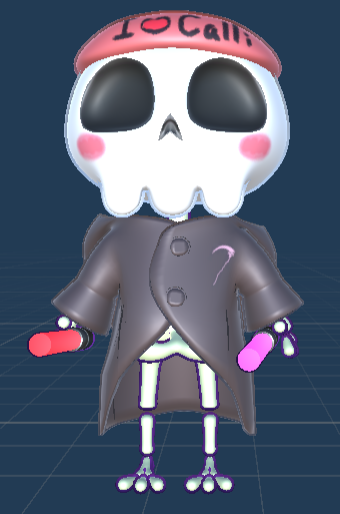
\includegraphics[width=0.2\textwidth]{images/deadbeat1.png}
		\caption{Deadbeat}
		\label{fig:deadbeat}
	\end{figure}
	
	\textbf{Description.} The most common enemy type in the game. These enemies rush toward the player's VTuber. On collision, they explode and deal a small amount of damage.

	\goodbreak

	\subsubsection{Smol Calli}

	\begin{figure}[H]
		\centering
		
\includegraphics[width=0.2\textwidth]{images/smol_calli1.png}
		\caption{Smol Calli}
		\label{fig:smolcalli}
	\end{figure}

	\textbf{Description.} The first ranged enemy type in the game. These enemies carry a homing missile. They launch the missile toward the player's VTuber and follow after it. If Smol Calli or the homing missile collide with the player's VTuber, they each explode and deal a small amount of damage.

	\subsubsection{Takodachi}

	\begin{figure}[H]
		\centering
		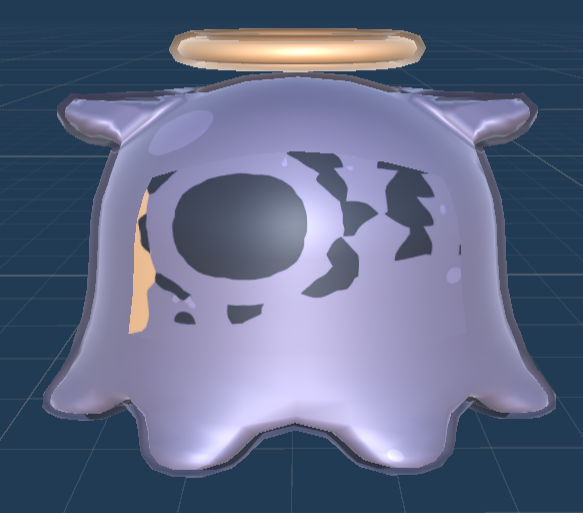
\includegraphics[width=0.2\textwidth]{images/takodachi1.png}
		\caption{Takodachi}
		\label{fig:takodachi}
	\end{figure}

	\textbf{Description.} A slow, bulky enemy characterized by high HP. These enemies move in a straight line. They don't go after the player's VTuber, but they deal high damage on collision. Otherwise, they disappear once they move past the edge of the screen.

	\subsubsection{Guy RyS}

	\begin{figure}[H]
		\centering
		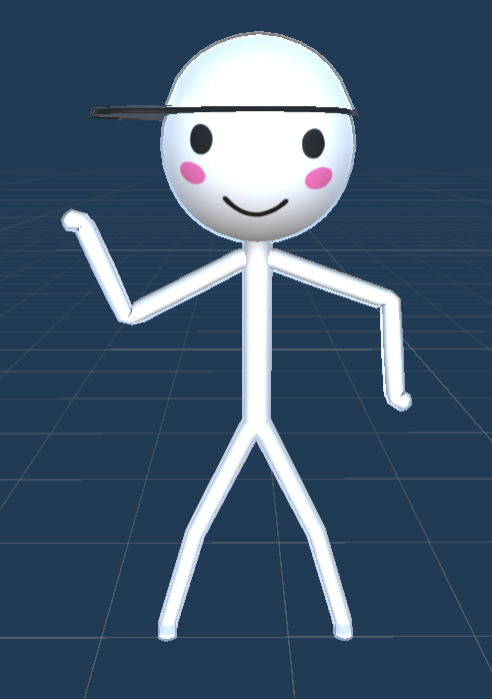
\includegraphics[width=0.2\textwidth]{images/guy_rys1.png}
		\caption{Guy RyS}
		\label{fig:guyrys}
	\end{figure}

	\textbf{Description.} A fast and lithe enemy that zips around the stage. These enemies don't go after the player's VTuber nor do they deal damage on collision. However, they intercept bullets from VTubers.

	\subsubsection{Smol Kiara}

	\begin{figure}[H]
		\centering
		
\includegraphics[width=0.2\textwidth]{images/smol_kiara1.png}
		\caption{Smol Kiara}
		\label{fig:smolkiara}
	\end{figure}

	\textbf{Description.} An enemy that only moves a short distance toward the player's VTuber upon spawning. Once she stops, she lunges at the the Vtuber, dealing moderate damage on collision.
	
	\subsubsection{Buff Ame}

	\begin{figure}[H]
		\centering
		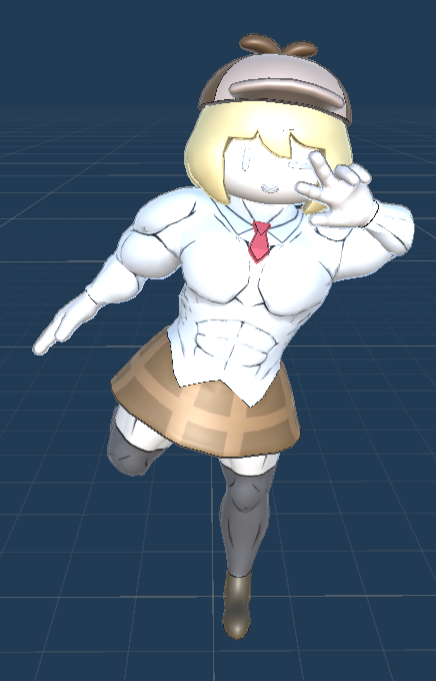
\includegraphics[width=0.2\textwidth]{images/buff_ame1.png}
		\caption{Buff Ame}
		\label{fig:buffame}
	\end{figure}

	\textbf{Description.} The boss of the first stage. Upon spawning, Buff Ame zips toward the center of the stage. Once Buff Ame has occupied its position, it moves horizontally back and forth. Buff Ame shoots projectiles that travel straight down the stage. On impact, these projectiles deal sizable damage. They move fast, too. Buff Ame's special attack spawns a number of missiles that home in toward the player's VTuber. Each missile deals a small amount of damage. Buff Ame has a respectable amount of HP for a first boss, and requires from the player a certain mastery over the mechanics of the game and their chosen VTuber to triumph.

	\subsubsection{Halloween Bae}

	\begin{figure}[H]
		\centering
		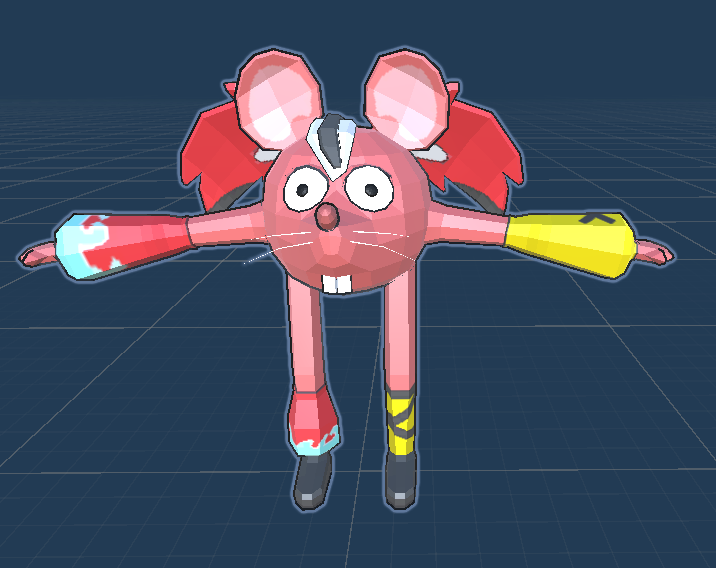
\includegraphics[width=0.2\textwidth]{images/halloween_bae1.png}
		\caption{Halloween Bae}
		\label{fig:halloweenbae}
	\end{figure}

	\textbf{Description.} The boss of the second stage. Halloween Bae zips erratically around the stage. It fires projectiles in a straight line continuously. Periodically, it spawns projectiles that home in toward the player.

	\subsubsection{Halloween Sana}

	\begin{figure}[H]
		\centering
		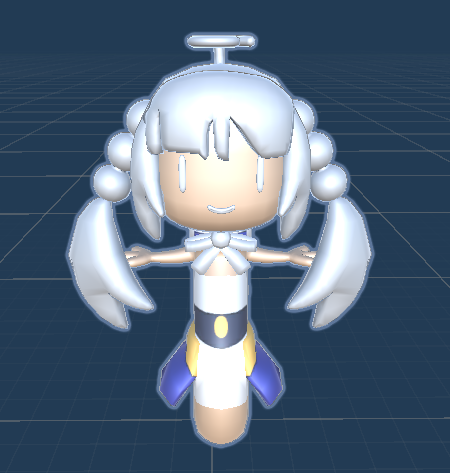
\includegraphics[width=0.2\textwidth]{images/halloween_sana1.png}
		\caption{Halloween Sana}
		\label{fig:halloweensana}
	\end{figure}

	\textbf{Description.} The boss of the third stage. Upon spawning, Halloween Sana moves toward a position away from the player. Once in position, she begins moving side to side. Periodically, she approaches the player while still moving side to side. After a brief period, she moves back to her original position. She fires bullets repeatedly at a constant rate. This pattern continues until she is defeated.

	\section{Appendix}

	The VShooter code repository is available at: \href{https://github.com/giociudadano/VShooter.git}{GitHub}. An asset tracker can be found at \href{https://docs.google.com/spreadsheets/d/1iixa0Slci229xnzVG4J9bXTK8P0FVPwnDIEXkRsuH7s/edit?usp=sharing}{Google Sheets}. VShooter remixes and the arranged sountrack can be downloaded from \href{https://drive.google.com/drive/folders/1lVz1maZ6dL9_K4PAbTF3IGDHxGWFrajg?usp=drive_link}{Drive}.

	\end{multicols}
\end{document}
